% Options for packages loaded elsewhere
\PassOptionsToPackage{unicode}{hyperref}
\PassOptionsToPackage{hyphens}{url}
%
\documentclass[
]{article}
\usepackage{lmodern}
\usepackage{amssymb,amsmath}
\usepackage{ifxetex,ifluatex}
\usepackage[hangul]{kotex}
\ifnum 0\ifxetex 1\fi\ifluatex 1\fi=0 % if pdftex
  \usepackage[T1]{fontenc}
  \usepackage[utf8]{inputenc}
  \usepackage{textcomp} % provide euro and other symbols
\else % if luatex or xetex
  \usepackage{unicode-math}
  \defaultfontfeatures{Scale=MatchLowercase}
  \defaultfontfeatures[\rmfamily]{Ligatures=TeX,Scale=1}
\fi
% Use upquote if available, for straight quotes in verbatim environments
\IfFileExists{upquote.sty}{\usepackage{upquote}}{}
\IfFileExists{microtype.sty}{% use microtype if available
  \usepackage[]{microtype}
  \UseMicrotypeSet[protrusion]{basicmath} % disable protrusion for tt fonts
}{}
\makeatletter
\@ifundefined{KOMAClassName}{% if non-KOMA class
  \IfFileExists{parskip.sty}{%
    \usepackage{parskip}
  }{% else
    \setlength{\parindent}{0pt}
    \setlength{\parskip}{6pt plus 2pt minus 1pt}}
}{% if KOMA class
  \KOMAoptions{parskip=half}}
\makeatother
\usepackage{xcolor}
\IfFileExists{xurl.sty}{\usepackage{xurl}}{} % add URL line breaks if available
\IfFileExists{bookmark.sty}{\usepackage{bookmark}}{\usepackage{hyperref}}
\hypersetup{
  pdftitle={Twin Studies on Smoking},
  pdfauthor={coop711},
  hidelinks,
  pdfcreator={LaTeX via pandoc}}
\urlstyle{same} % disable monospaced font for URLs
\usepackage[margin=1in]{geometry}
\usepackage{color}
\usepackage{fancyvrb}
\newcommand{\VerbBar}{|}
\newcommand{\VERB}{\Verb[commandchars=\\\{\}]}
\DefineVerbatimEnvironment{Highlighting}{Verbatim}{commandchars=\\\{\}}
% Add ',fontsize=\small' for more characters per line
\usepackage{framed}
\definecolor{shadecolor}{RGB}{248,248,248}
\newenvironment{Shaded}{\begin{snugshade}}{\end{snugshade}}
\newcommand{\AlertTok}[1]{\textcolor[rgb]{0.94,0.16,0.16}{#1}}
\newcommand{\AnnotationTok}[1]{\textcolor[rgb]{0.56,0.35,0.01}{\textbf{\textit{#1}}}}
\newcommand{\AttributeTok}[1]{\textcolor[rgb]{0.77,0.63,0.00}{#1}}
\newcommand{\BaseNTok}[1]{\textcolor[rgb]{0.00,0.00,0.81}{#1}}
\newcommand{\BuiltInTok}[1]{#1}
\newcommand{\CharTok}[1]{\textcolor[rgb]{0.31,0.60,0.02}{#1}}
\newcommand{\CommentTok}[1]{\textcolor[rgb]{0.56,0.35,0.01}{\textit{#1}}}
\newcommand{\CommentVarTok}[1]{\textcolor[rgb]{0.56,0.35,0.01}{\textbf{\textit{#1}}}}
\newcommand{\ConstantTok}[1]{\textcolor[rgb]{0.00,0.00,0.00}{#1}}
\newcommand{\ControlFlowTok}[1]{\textcolor[rgb]{0.13,0.29,0.53}{\textbf{#1}}}
\newcommand{\DataTypeTok}[1]{\textcolor[rgb]{0.13,0.29,0.53}{#1}}
\newcommand{\DecValTok}[1]{\textcolor[rgb]{0.00,0.00,0.81}{#1}}
\newcommand{\DocumentationTok}[1]{\textcolor[rgb]{0.56,0.35,0.01}{\textbf{\textit{#1}}}}
\newcommand{\ErrorTok}[1]{\textcolor[rgb]{0.64,0.00,0.00}{\textbf{#1}}}
\newcommand{\ExtensionTok}[1]{#1}
\newcommand{\FloatTok}[1]{\textcolor[rgb]{0.00,0.00,0.81}{#1}}
\newcommand{\FunctionTok}[1]{\textcolor[rgb]{0.00,0.00,0.00}{#1}}
\newcommand{\ImportTok}[1]{#1}
\newcommand{\InformationTok}[1]{\textcolor[rgb]{0.56,0.35,0.01}{\textbf{\textit{#1}}}}
\newcommand{\KeywordTok}[1]{\textcolor[rgb]{0.13,0.29,0.53}{\textbf{#1}}}
\newcommand{\NormalTok}[1]{#1}
\newcommand{\OperatorTok}[1]{\textcolor[rgb]{0.81,0.36,0.00}{\textbf{#1}}}
\newcommand{\OtherTok}[1]{\textcolor[rgb]{0.56,0.35,0.01}{#1}}
\newcommand{\PreprocessorTok}[1]{\textcolor[rgb]{0.56,0.35,0.01}{\textit{#1}}}
\newcommand{\RegionMarkerTok}[1]{#1}
\newcommand{\SpecialCharTok}[1]{\textcolor[rgb]{0.00,0.00,0.00}{#1}}
\newcommand{\SpecialStringTok}[1]{\textcolor[rgb]{0.31,0.60,0.02}{#1}}
\newcommand{\StringTok}[1]{\textcolor[rgb]{0.31,0.60,0.02}{#1}}
\newcommand{\VariableTok}[1]{\textcolor[rgb]{0.00,0.00,0.00}{#1}}
\newcommand{\VerbatimStringTok}[1]{\textcolor[rgb]{0.31,0.60,0.02}{#1}}
\newcommand{\WarningTok}[1]{\textcolor[rgb]{0.56,0.35,0.01}{\textbf{\textit{#1}}}}
\usepackage{graphicx,grffile}
\makeatletter
\def\maxwidth{\ifdim\Gin@nat@width>\linewidth\linewidth\else\Gin@nat@width\fi}
\def\maxheight{\ifdim\Gin@nat@height>\textheight\textheight\else\Gin@nat@height\fi}
\makeatother
% Scale images if necessary, so that they will not overflow the page
% margins by default, and it is still possible to overwrite the defaults
% using explicit options in \includegraphics[width, height, ...]{}
\setkeys{Gin}{width=\maxwidth,height=\maxheight,keepaspectratio}
% Set default figure placement to htbp
\makeatletter
\def\fps@figure{htbp}
\makeatother
\setlength{\emergencystretch}{3em} % prevent overfull lines
\providecommand{\tightlist}{%
  \setlength{\itemsep}{0pt}\setlength{\parskip}{0pt}}
\setcounter{secnumdepth}{-\maxdimen} % remove section numbering

\title{Twin Studies on Smoking}
\author{coop711}
\date{2021-02-10}

\begin{document}
\maketitle

\begin{Shaded}
\begin{Highlighting}[]
\KeywordTok{library}\NormalTok{(magrittr)}
\KeywordTok{library}\NormalTok{(tidyverse)}
\CommentTok{# par(mfrow = c(1, 2))}
\CommentTok{#> 제시된 표와 닮은 행열 생성}
\NormalTok{Nature1 <-}\StringTok{ }\KeywordTok{matrix}\NormalTok{(}\KeywordTok{c}\NormalTok{(}\DecValTok{1}\NormalTok{, }\DecValTok{1}\NormalTok{, }\DecValTok{1}\NormalTok{, }\DecValTok{3}\NormalTok{, }\DecValTok{1}\NormalTok{, }\DecValTok{9}\NormalTok{), }
                  \DataTypeTok{nrow =} \DecValTok{3}\NormalTok{, }\DataTypeTok{byrow =} \OtherTok{TRUE}\NormalTok{)}
\KeywordTok{rownames}\NormalTok{(Nature1) <-}\StringTok{ }\KeywordTok{c}\NormalTok{(}\StringTok{"1990"}\NormalTok{, }\StringTok{"2000"}\NormalTok{, }\StringTok{"2010"}\NormalTok{)}
\KeywordTok{colnames}\NormalTok{(Nature1) <-}\StringTok{ }\KeywordTok{c}\NormalTok{(}\StringTok{"시골"}\NormalTok{, }\StringTok{"서울"}\NormalTok{)}
\NormalTok{Nature1}
\end{Highlighting}
\end{Shaded}

\begin{verbatim}
##      시골 서울
## 1990    1    1
## 2000    1    3
## 2010    1    9
\end{verbatim}

\hypertarget{uxd589uxb82c-uxad6cuxc870uxc640-barplot}{%
\paragraph{행렬 구조와
barplot}\label{uxd589uxb82c-uxad6cuxc870uxc640-barplot}}

\begin{Shaded}
\begin{Highlighting}[]
\NormalTok{Nature1 }\OperatorTok
\StringTok{  }\NormalTok{barplot}
\end{Highlighting}
\end{Shaded}

\begin{verbatim}
## Warning in axis(if (horiz) 2 else 1, at = at.l, labels = names.arg, lty =
## axis.lty, : conversion failure on '시골' in 'mbcsToSbcs': dot substituted for
## <ec>
\end{verbatim}

\begin{verbatim}
## Warning in axis(if (horiz) 2 else 1, at = at.l, labels = names.arg, lty =
## axis.lty, : conversion failure on '시골' in 'mbcsToSbcs': dot substituted for
## <8b>
\end{verbatim}

\begin{verbatim}
## Warning in axis(if (horiz) 2 else 1, at = at.l, labels = names.arg, lty =
## axis.lty, : conversion failure on '시골' in 'mbcsToSbcs': dot substituted for
## <9c>
\end{verbatim}

\begin{verbatim}
## Warning in axis(if (horiz) 2 else 1, at = at.l, labels = names.arg, lty =
## axis.lty, : conversion failure on '시골' in 'mbcsToSbcs': dot substituted for
## <ea>
\end{verbatim}

\begin{verbatim}
## Warning in axis(if (horiz) 2 else 1, at = at.l, labels = names.arg, lty =
## axis.lty, : conversion failure on '시골' in 'mbcsToSbcs': dot substituted for
## <b3>
\end{verbatim}

\begin{verbatim}
## Warning in axis(if (horiz) 2 else 1, at = at.l, labels = names.arg, lty =
## axis.lty, : conversion failure on '시골' in 'mbcsToSbcs': dot substituted for
## <a8>
\end{verbatim}

\begin{verbatim}
## Warning in axis(if (horiz) 2 else 1, at = at.l, labels = names.arg, lty =
## axis.lty, : conversion failure on '시골' in 'mbcsToSbcs': dot substituted for
## <ec>
\end{verbatim}

\begin{verbatim}
## Warning in axis(if (horiz) 2 else 1, at = at.l, labels = names.arg, lty =
## axis.lty, : conversion failure on '시골' in 'mbcsToSbcs': dot substituted for
## <8b>
\end{verbatim}

\begin{verbatim}
## Warning in axis(if (horiz) 2 else 1, at = at.l, labels = names.arg, lty =
## axis.lty, : conversion failure on '시골' in 'mbcsToSbcs': dot substituted for
## <9c>
\end{verbatim}

\begin{verbatim}
## Warning in axis(if (horiz) 2 else 1, at = at.l, labels = names.arg, lty =
## axis.lty, : conversion failure on '시골' in 'mbcsToSbcs': dot substituted for
## <ea>
\end{verbatim}

\begin{verbatim}
## Warning in axis(if (horiz) 2 else 1, at = at.l, labels = names.arg, lty =
## axis.lty, : conversion failure on '시골' in 'mbcsToSbcs': dot substituted for
## <b3>
\end{verbatim}

\begin{verbatim}
## Warning in axis(if (horiz) 2 else 1, at = at.l, labels = names.arg, lty =
## axis.lty, : conversion failure on '시골' in 'mbcsToSbcs': dot substituted for
## <a8>
\end{verbatim}

\begin{verbatim}
## Warning in axis(if (horiz) 2 else 1, at = at.l, labels = names.arg, lty =
## axis.lty, : conversion failure on '서울' in 'mbcsToSbcs': dot substituted for
## <ec>
\end{verbatim}

\begin{verbatim}
## Warning in axis(if (horiz) 2 else 1, at = at.l, labels = names.arg, lty =
## axis.lty, : conversion failure on '서울' in 'mbcsToSbcs': dot substituted for
## <84>
\end{verbatim}

\begin{verbatim}
## Warning in axis(if (horiz) 2 else 1, at = at.l, labels = names.arg, lty =
## axis.lty, : conversion failure on '서울' in 'mbcsToSbcs': dot substituted for
## <9c>
\end{verbatim}

\begin{verbatim}
## Warning in axis(if (horiz) 2 else 1, at = at.l, labels = names.arg, lty =
## axis.lty, : conversion failure on '서울' in 'mbcsToSbcs': dot substituted for
## <ec>
\end{verbatim}

\begin{verbatim}
## Warning in axis(if (horiz) 2 else 1, at = at.l, labels = names.arg, lty =
## axis.lty, : conversion failure on '서울' in 'mbcsToSbcs': dot substituted for
## <9a>
\end{verbatim}

\begin{verbatim}
## Warning in axis(if (horiz) 2 else 1, at = at.l, labels = names.arg, lty =
## axis.lty, : conversion failure on '서울' in 'mbcsToSbcs': dot substituted for
## <b8>
\end{verbatim}

\begin{verbatim}
## Warning in axis(if (horiz) 2 else 1, at = at.l, labels = names.arg, lty =
## axis.lty, : conversion failure on '서울' in 'mbcsToSbcs': dot substituted for
## <ec>
\end{verbatim}

\begin{verbatim}
## Warning in axis(if (horiz) 2 else 1, at = at.l, labels = names.arg, lty =
## axis.lty, : conversion failure on '서울' in 'mbcsToSbcs': dot substituted for
## <84>
\end{verbatim}

\begin{verbatim}
## Warning in axis(if (horiz) 2 else 1, at = at.l, labels = names.arg, lty =
## axis.lty, : conversion failure on '서울' in 'mbcsToSbcs': dot substituted for
## <9c>
\end{verbatim}

\begin{verbatim}
## Warning in axis(if (horiz) 2 else 1, at = at.l, labels = names.arg, lty =
## axis.lty, : conversion failure on '서울' in 'mbcsToSbcs': dot substituted for
## <ec>
\end{verbatim}

\begin{verbatim}
## Warning in axis(if (horiz) 2 else 1, at = at.l, labels = names.arg, lty =
## axis.lty, : conversion failure on '서울' in 'mbcsToSbcs': dot substituted for
## <9a>
\end{verbatim}

\begin{verbatim}
## Warning in axis(if (horiz) 2 else 1, at = at.l, labels = names.arg, lty =
## axis.lty, : conversion failure on '서울' in 'mbcsToSbcs': dot substituted for
## <b8>
\end{verbatim}

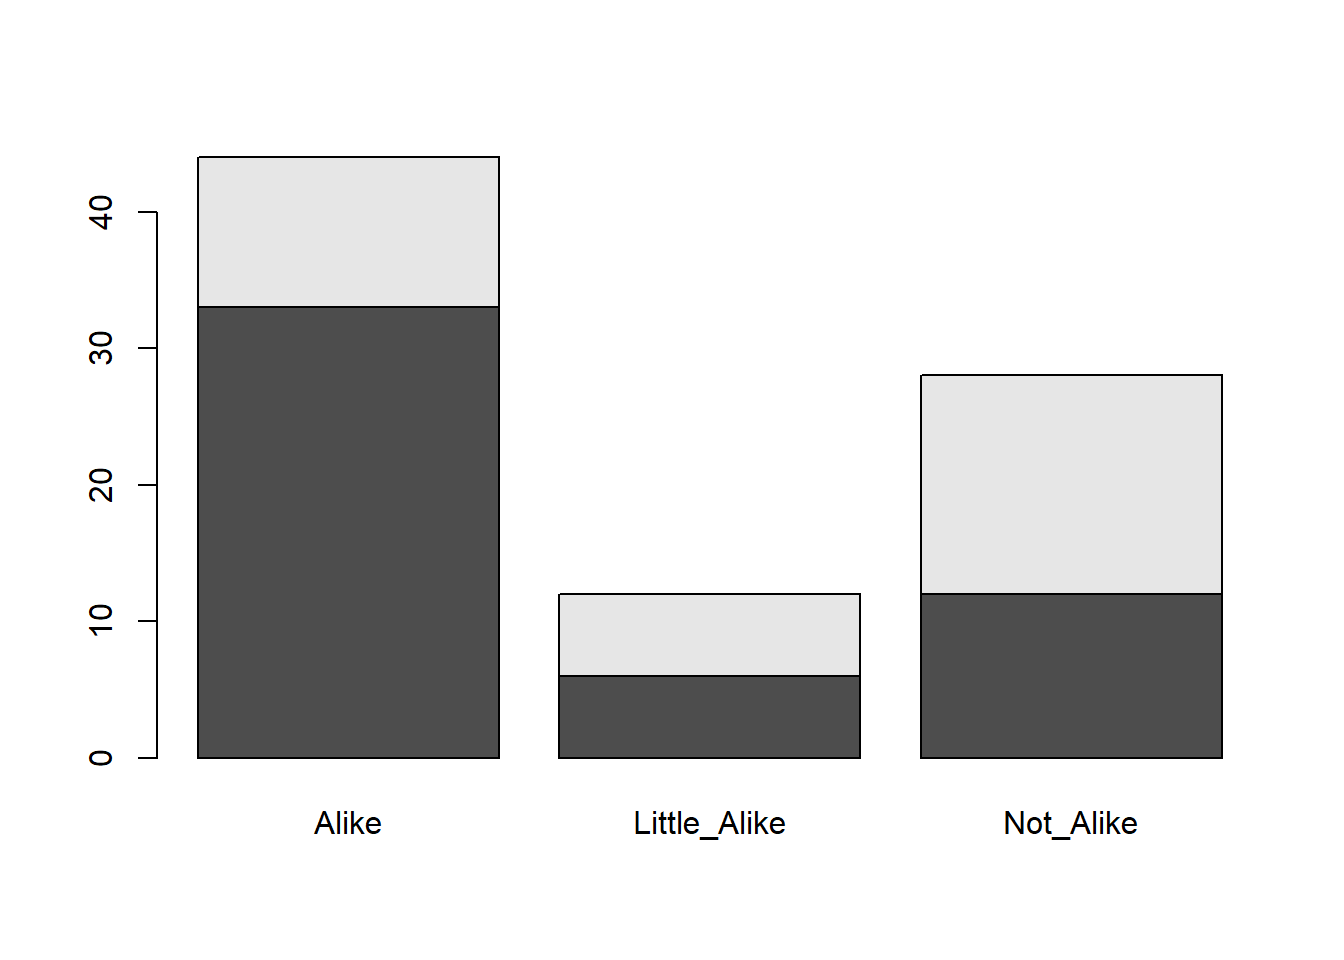
\includegraphics[width=0.5\linewidth]{Inequality_files/figure-latex/unnamed-chunk-2-1}

\begin{Shaded}
\begin{Highlighting}[]
\NormalTok{Nature1 }\OperatorTok\StringTok{ }
\StringTok{  }\NormalTok{t }\OperatorTok
\StringTok{  }\NormalTok{barplot}
\end{Highlighting}
\end{Shaded}

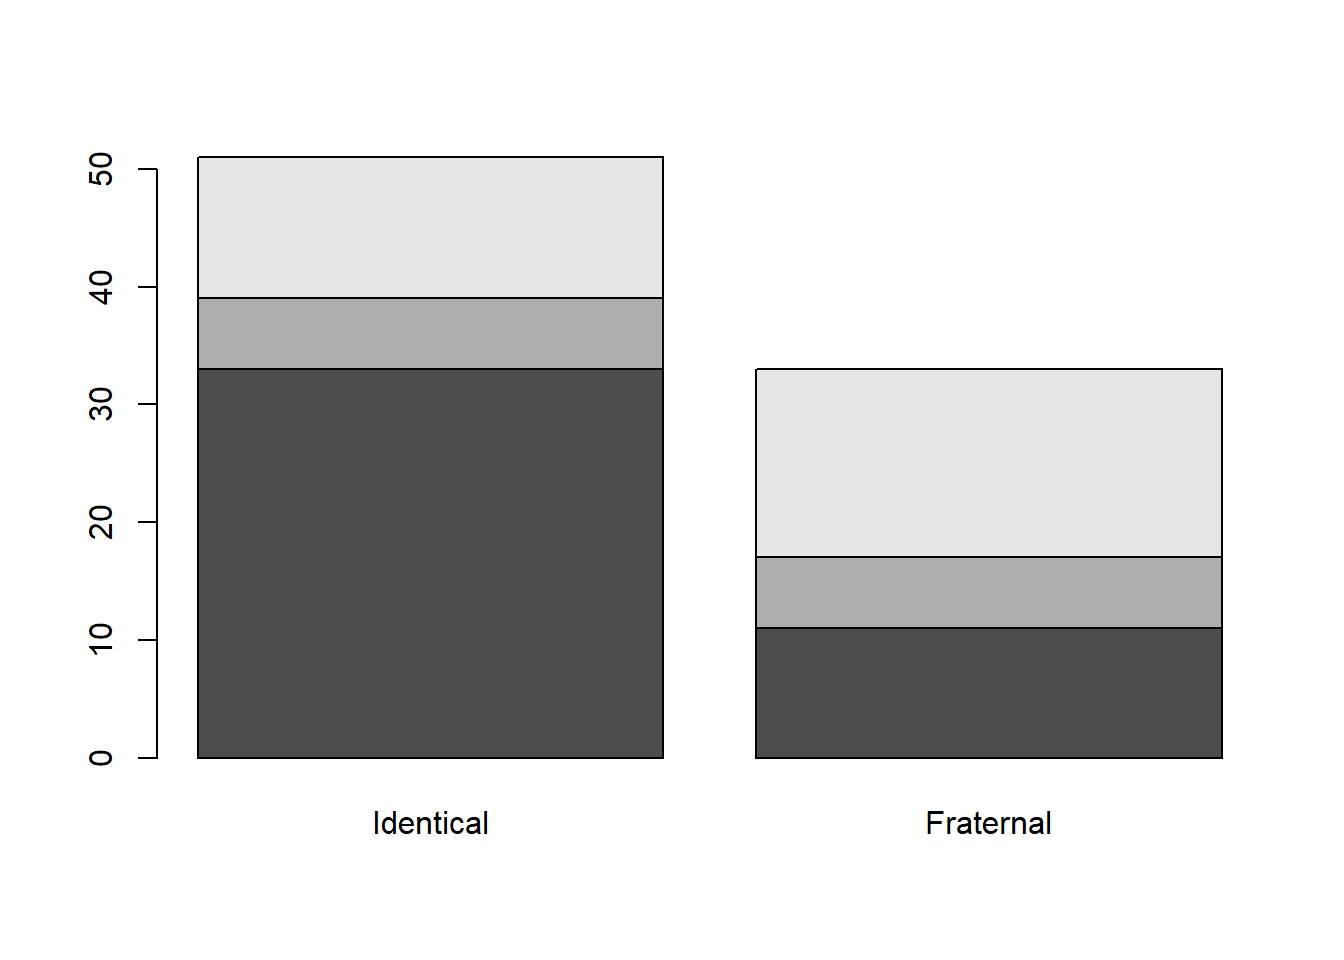
\includegraphics[width=0.5\linewidth]{Inequality_files/figure-latex/unnamed-chunk-2-2}

\begin{Shaded}
\begin{Highlighting}[]
\CommentTok{# par(mfrow = c(1, 1))}
\end{Highlighting}
\end{Shaded}

\texttt{Nature1}의 구조를 전치(transpose)해 주어야 원하는 모양의
막대그래프가 나올 것임을 알 수 있다. 나머지 이러한 점을 염두에 두고
작성한다.

\hypertarget{stack}{%
\subsubsection{Stack}\label{stack}}

\begin{Shaded}
\begin{Highlighting}[]
\KeywordTok{options}\NormalTok{(}\DataTypeTok{digits =} \DecValTok{3}\NormalTok{)}
\CommentTok{#> RColorBrewer 패키지를 이용하여 컬러 생성}
\KeywordTok{library}\NormalTok{(RColorBrewer)}
\CommentTok{#> "Accent" palette 채택}
\NormalTok{cols <-}\StringTok{ }\KeywordTok{brewer.pal}\NormalTok{(}\DecValTok{8}\NormalTok{, }\StringTok{"Accent"}\NormalTok{)}
\CommentTok{#> 막대의 가운데에 추가 정보를 넣기 위한 좌표 설정 함수. }
\CommentTok{# pos <- function(x)\{}
\CommentTok{#   cumsum(x) - x / 2}
\CommentTok{# \}}
\NormalTok{pos <-}\StringTok{ }\NormalTok{. }\OperatorTok\StringTok{ }\NormalTok{\{}\StringTok{`}\DataTypeTok{-}\StringTok{`}\NormalTok{(}\KeywordTok{cumsum}\NormalTok{(.), . }\OperatorTok{/}\StringTok{ }\DecValTok{2}\NormalTok{)\}}
\CommentTok{# pos <- . %>% \{cumsum(.) - . / 2\}}
\CommentTok{#> 아래와 같이 작성하면 오류 발생}
\CommentTok{# pos <- . %>% cumsum(.) - . / 2}
\CommentTok{#> 텍스트 정보 넣을 좌표를 계산한다. }
\NormalTok{y1_text <-}\StringTok{ }\KeywordTok{apply}\NormalTok{(Nature1, }
                 \DataTypeTok{MARGIN =} \DecValTok{1}\NormalTok{, }
                 \DataTypeTok{FUN =}\NormalTok{ pos)}
\end{Highlighting}
\end{Shaded}

\begin{Shaded}
\begin{Highlighting}[]
\CommentTok{# par(family = "KoPubWorldDotum Medium")}
\NormalTok{b1 <-}\StringTok{ }\NormalTok{Nature1 }\OperatorTok\StringTok{ }
\StringTok{  }\NormalTok{t }\OperatorTok
\StringTok{  }\KeywordTok{barplot}\NormalTok{(}\DataTypeTok{width =} \FloatTok{0.8}\NormalTok{, }
          \DataTypeTok{xlim =} \KeywordTok{c}\NormalTok{(}\DecValTok{0}\NormalTok{, }\DecValTok{5}\NormalTok{), }
          \DataTypeTok{space =} \DecValTok{1}\NormalTok{, }
          \DataTypeTok{col =}\NormalTok{ cols[}\DecValTok{1}\OperatorTok{:}\DecValTok{2}\NormalTok{], }
          \DataTypeTok{yaxt =} \StringTok{"n"}\NormalTok{)}
\CommentTok{#> 쌍둥이유형 별로 한 막대에 흡연습관의 닮음 정도를 나타낼 것이므로 `cumsum`함수를 이용하여 막대들이 위치할 좌표를 계산한다. 일란성과 이란성 각각의 수효부터 비교할 수 있도록  막대 높이로 나타내고, 막대 중심에는 해당 속성의 돗수를 표시한다. 원점을 나타내기 위하여 0을 `c`함수 안에 추가하였다. 이를 추가하지 않으면 축이 어떻게 표시되는지 비교한다.}
\CommentTok{#> `format`함수의 용법에 익숙해지고, `las = 2`가 왜 필요한지 여러 경우를 비교하라.}
\KeywordTok{axis}\NormalTok{(}\DataTypeTok{side =} \DecValTok{2}\NormalTok{,}
     \DataTypeTok{at =} \KeywordTok{c}\NormalTok{(}\DecValTok{0}\NormalTok{, }\KeywordTok{apply}\NormalTok{(}\KeywordTok{t}\NormalTok{(Nature1),}
                     \DataTypeTok{MARGIN =} \DecValTok{2}\NormalTok{, }
                     \DataTypeTok{FUN =}\NormalTok{ cumsum)),}
     \DataTypeTok{labels =} \KeywordTok{format}\NormalTok{(}\KeywordTok{c}\NormalTok{(}\DecValTok{0}\NormalTok{, }\KeywordTok{apply}\NormalTok{(}\KeywordTok{t}\NormalTok{(Nature1), }
                                \DataTypeTok{MARGIN =} \DecValTok{2}\NormalTok{, }
                                \DataTypeTok{FUN =}\NormalTok{ cumsum)), }
                     \DataTypeTok{digits =} \DecValTok{3}\NormalTok{, }
                     \DataTypeTok{nsmall =} \DecValTok{0}\NormalTok{), }
     \DataTypeTok{las =} \DecValTok{2}\NormalTok{)}
\KeywordTok{mtext}\NormalTok{(}\DataTypeTok{text =} \StringTok{"단위(억원)"}\NormalTok{, }\DataTypeTok{side =} \DecValTok{2}\NormalTok{, }\DataTypeTok{at =} \DecValTok{11}\NormalTok{, }\DataTypeTok{las =} \DecValTok{2}\NormalTok{)}
\end{Highlighting}
\end{Shaded}

\begin{verbatim}
## Warning in mtext(text = "단위(억원)", side = 2, at = 11, las = 2): conversion
## failure on '단위(억원)' in 'mbcsToSbcs': dot substituted for <eb>
\end{verbatim}

\begin{verbatim}
## Warning in mtext(text = "단위(억원)", side = 2, at = 11, las = 2): conversion
## failure on '단위(억원)' in 'mbcsToSbcs': dot substituted for <8b>
\end{verbatim}

\begin{verbatim}
## Warning in mtext(text = "단위(억원)", side = 2, at = 11, las = 2): conversion
## failure on '단위(억원)' in 'mbcsToSbcs': dot substituted for <a8>
\end{verbatim}

\begin{verbatim}
## Warning in mtext(text = "단위(억원)", side = 2, at = 11, las = 2): conversion
## failure on '단위(억원)' in 'mbcsToSbcs': dot substituted for <ec>
\end{verbatim}

\begin{verbatim}
## Warning in mtext(text = "단위(억원)", side = 2, at = 11, las = 2): conversion
## failure on '단위(억원)' in 'mbcsToSbcs': dot substituted for <9c>
\end{verbatim}

\begin{verbatim}
## Warning in mtext(text = "단위(억원)", side = 2, at = 11, las = 2): conversion
## failure on '단위(억원)' in 'mbcsToSbcs': dot substituted for <84>
\end{verbatim}

\begin{verbatim}
## Warning in mtext(text = "단위(억원)", side = 2, at = 11, las = 2): conversion
## failure on '단위(억원)' in 'mbcsToSbcs': dot substituted for <ec>
\end{verbatim}

\begin{verbatim}
## Warning in mtext(text = "단위(억원)", side = 2, at = 11, las = 2): conversion
## failure on '단위(억원)' in 'mbcsToSbcs': dot substituted for <96>
\end{verbatim}

\begin{verbatim}
## Warning in mtext(text = "단위(억원)", side = 2, at = 11, las = 2): conversion
## failure on '단위(억원)' in 'mbcsToSbcs': dot substituted for <b5>
\end{verbatim}

\begin{verbatim}
## Warning in mtext(text = "단위(억원)", side = 2, at = 11, las = 2): conversion
## failure on '단위(억원)' in 'mbcsToSbcs': dot substituted for <ec>
\end{verbatim}

\begin{verbatim}
## Warning in mtext(text = "단위(억원)", side = 2, at = 11, las = 2): conversion
## failure on '단위(억원)' in 'mbcsToSbcs': dot substituted for <9b>
\end{verbatim}

\begin{verbatim}
## Warning in mtext(text = "단위(억원)", side = 2, at = 11, las = 2): conversion
## failure on '단위(억원)' in 'mbcsToSbcs': dot substituted for <90>
\end{verbatim}

\begin{Shaded}
\begin{Highlighting}[]
\CommentTok{#> 막대그래프 작성 과정에서 나온 막대의 좌표와 `pos`함수로 계산한 y좌표를 이용하여 실제 관찰된 쌍둥이 페어의 수효를 표시한다.`y_text`의 구조에 맞추어 `rep()`에서 `each = 3`으로 설정하였다. `bty = ` `"o" 또는 "n"으로 정할 수 있다. }
\KeywordTok{text}\NormalTok{(}\DataTypeTok{x =} \KeywordTok{rep}\NormalTok{(b1, }\DataTypeTok{each =} \DecValTok{2}\NormalTok{), }
     \DataTypeTok{y =}\NormalTok{ y1_text, }
     \DataTypeTok{labels =} \KeywordTok{paste0}\NormalTok{(}\KeywordTok{t}\NormalTok{(Nature1), }\StringTok{"억"}\NormalTok{))}
\end{Highlighting}
\end{Shaded}

\begin{verbatim}
## Warning in text.default(x = rep(b1, each = 2), y = y1_text, labels =
## paste0(t(Nature1), : conversion failure on '1억' in 'mbcsToSbcs': dot
## substituted for <ec>
\end{verbatim}

\begin{verbatim}
## Warning in text.default(x = rep(b1, each = 2), y = y1_text, labels =
## paste0(t(Nature1), : conversion failure on '1억' in 'mbcsToSbcs': dot
## substituted for <96>
\end{verbatim}

\begin{verbatim}
## Warning in text.default(x = rep(b1, each = 2), y = y1_text, labels =
## paste0(t(Nature1), : conversion failure on '1억' in 'mbcsToSbcs': dot
## substituted for <b5>
\end{verbatim}

\begin{verbatim}
## Warning in text.default(x = rep(b1, each = 2), y = y1_text, labels =
## paste0(t(Nature1), : font metrics unknown for Unicode character U+c5b5
\end{verbatim}

\begin{verbatim}
## Warning in text.default(x = rep(b1, each = 2), y = y1_text, labels =
## paste0(t(Nature1), : conversion failure on '1억' in 'mbcsToSbcs': dot
## substituted for <ec>
\end{verbatim}

\begin{verbatim}
## Warning in text.default(x = rep(b1, each = 2), y = y1_text, labels =
## paste0(t(Nature1), : conversion failure on '1억' in 'mbcsToSbcs': dot
## substituted for <96>
\end{verbatim}

\begin{verbatim}
## Warning in text.default(x = rep(b1, each = 2), y = y1_text, labels =
## paste0(t(Nature1), : conversion failure on '1억' in 'mbcsToSbcs': dot
## substituted for <b5>
\end{verbatim}

\begin{verbatim}
## Warning in text.default(x = rep(b1, each = 2), y = y1_text, labels =
## paste0(t(Nature1), : font metrics unknown for Unicode character U+c5b5
\end{verbatim}

\begin{verbatim}
## Warning in text.default(x = rep(b1, each = 2), y = y1_text, labels =
## paste0(t(Nature1), : conversion failure on '1억' in 'mbcsToSbcs': dot
## substituted for <ec>
\end{verbatim}

\begin{verbatim}
## Warning in text.default(x = rep(b1, each = 2), y = y1_text, labels =
## paste0(t(Nature1), : conversion failure on '1억' in 'mbcsToSbcs': dot
## substituted for <96>
\end{verbatim}

\begin{verbatim}
## Warning in text.default(x = rep(b1, each = 2), y = y1_text, labels =
## paste0(t(Nature1), : conversion failure on '1억' in 'mbcsToSbcs': dot
## substituted for <b5>
\end{verbatim}

\begin{verbatim}
## Warning in text.default(x = rep(b1, each = 2), y = y1_text, labels =
## paste0(t(Nature1), : font metrics unknown for Unicode character U+c5b5
\end{verbatim}

\begin{verbatim}
## Warning in text.default(x = rep(b1, each = 2), y = y1_text, labels =
## paste0(t(Nature1), : conversion failure on '3억' in 'mbcsToSbcs': dot
## substituted for <ec>
\end{verbatim}

\begin{verbatim}
## Warning in text.default(x = rep(b1, each = 2), y = y1_text, labels =
## paste0(t(Nature1), : conversion failure on '3억' in 'mbcsToSbcs': dot
## substituted for <96>
\end{verbatim}

\begin{verbatim}
## Warning in text.default(x = rep(b1, each = 2), y = y1_text, labels =
## paste0(t(Nature1), : conversion failure on '3억' in 'mbcsToSbcs': dot
## substituted for <b5>
\end{verbatim}

\begin{verbatim}
## Warning in text.default(x = rep(b1, each = 2), y = y1_text, labels =
## paste0(t(Nature1), : font metrics unknown for Unicode character U+c5b5
\end{verbatim}

\begin{verbatim}
## Warning in text.default(x = rep(b1, each = 2), y = y1_text, labels =
## paste0(t(Nature1), : conversion failure on '1억' in 'mbcsToSbcs': dot
## substituted for <ec>
\end{verbatim}

\begin{verbatim}
## Warning in text.default(x = rep(b1, each = 2), y = y1_text, labels =
## paste0(t(Nature1), : conversion failure on '1억' in 'mbcsToSbcs': dot
## substituted for <96>
\end{verbatim}

\begin{verbatim}
## Warning in text.default(x = rep(b1, each = 2), y = y1_text, labels =
## paste0(t(Nature1), : conversion failure on '1억' in 'mbcsToSbcs': dot
## substituted for <b5>
\end{verbatim}

\begin{verbatim}
## Warning in text.default(x = rep(b1, each = 2), y = y1_text, labels =
## paste0(t(Nature1), : font metrics unknown for Unicode character U+c5b5
\end{verbatim}

\begin{verbatim}
## Warning in text.default(x = rep(b1, each = 2), y = y1_text, labels =
## paste0(t(Nature1), : conversion failure on '9억' in 'mbcsToSbcs': dot
## substituted for <ec>
\end{verbatim}

\begin{verbatim}
## Warning in text.default(x = rep(b1, each = 2), y = y1_text, labels =
## paste0(t(Nature1), : conversion failure on '9억' in 'mbcsToSbcs': dot
## substituted for <96>
\end{verbatim}

\begin{verbatim}
## Warning in text.default(x = rep(b1, each = 2), y = y1_text, labels =
## paste0(t(Nature1), : conversion failure on '9억' in 'mbcsToSbcs': dot
## substituted for <b5>
\end{verbatim}

\begin{verbatim}
## Warning in text.default(x = rep(b1, each = 2), y = y1_text, labels =
## paste0(t(Nature1), : font metrics unknown for Unicode character U+c5b5
\end{verbatim}

\begin{Shaded}
\begin{Highlighting}[]
\CommentTok{#> 범례 표시}
\KeywordTok{legend}\NormalTok{(}\StringTok{"topleft"}\NormalTok{, }
       \DataTypeTok{inset =} \FloatTok{0.01}\NormalTok{, }
       \DataTypeTok{fill =}\NormalTok{ cols[}\DecValTok{2}\OperatorTok{:}\DecValTok{1}\NormalTok{], }
       \DataTypeTok{legend =} \KeywordTok{rev}\NormalTok{(}\KeywordTok{colnames}\NormalTok{(Nature1)), }
       \DataTypeTok{bty =} \StringTok{"n"}\NormalTok{)}
\end{Highlighting}
\end{Shaded}

\begin{verbatim}
## Warning in strwidth(legend, units = "user", cex = cex, font = text.font):
## conversion failure on '서울' in 'mbcsToSbcs': dot substituted for <ec>
\end{verbatim}

\begin{verbatim}
## Warning in strwidth(legend, units = "user", cex = cex, font = text.font):
## conversion failure on '서울' in 'mbcsToSbcs': dot substituted for <84>
\end{verbatim}

\begin{verbatim}
## Warning in strwidth(legend, units = "user", cex = cex, font = text.font):
## conversion failure on '서울' in 'mbcsToSbcs': dot substituted for <9c>
\end{verbatim}

\begin{verbatim}
## Warning in strwidth(legend, units = "user", cex = cex, font = text.font):
## conversion failure on '서울' in 'mbcsToSbcs': dot substituted for <ec>
\end{verbatim}

\begin{verbatim}
## Warning in strwidth(legend, units = "user", cex = cex, font = text.font):
## conversion failure on '서울' in 'mbcsToSbcs': dot substituted for <9a>
\end{verbatim}

\begin{verbatim}
## Warning in strwidth(legend, units = "user", cex = cex, font = text.font):
## conversion failure on '서울' in 'mbcsToSbcs': dot substituted for <b8>
\end{verbatim}

\begin{verbatim}
## Warning in strwidth(legend, units = "user", cex = cex, font = text.font):
## conversion failure on '시골' in 'mbcsToSbcs': dot substituted for <ec>
\end{verbatim}

\begin{verbatim}
## Warning in strwidth(legend, units = "user", cex = cex, font = text.font):
## conversion failure on '시골' in 'mbcsToSbcs': dot substituted for <8b>
\end{verbatim}

\begin{verbatim}
## Warning in strwidth(legend, units = "user", cex = cex, font = text.font):
## conversion failure on '시골' in 'mbcsToSbcs': dot substituted for <9c>
\end{verbatim}

\begin{verbatim}
## Warning in strwidth(legend, units = "user", cex = cex, font = text.font):
## conversion failure on '시골' in 'mbcsToSbcs': dot substituted for <ea>
\end{verbatim}

\begin{verbatim}
## Warning in strwidth(legend, units = "user", cex = cex, font = text.font):
## conversion failure on '시골' in 'mbcsToSbcs': dot substituted for <b3>
\end{verbatim}

\begin{verbatim}
## Warning in strwidth(legend, units = "user", cex = cex, font = text.font):
## conversion failure on '시골' in 'mbcsToSbcs': dot substituted for <a8>
\end{verbatim}

\begin{verbatim}
## Warning in text.default(x, y, ...): conversion failure on '서울' in
## 'mbcsToSbcs': dot substituted for <ec>
\end{verbatim}

\begin{verbatim}
## Warning in text.default(x, y, ...): conversion failure on '서울' in
## 'mbcsToSbcs': dot substituted for <84>
\end{verbatim}

\begin{verbatim}
## Warning in text.default(x, y, ...): conversion failure on '서울' in
## 'mbcsToSbcs': dot substituted for <9c>
\end{verbatim}

\begin{verbatim}
## Warning in text.default(x, y, ...): conversion failure on '서울' in
## 'mbcsToSbcs': dot substituted for <ec>
\end{verbatim}

\begin{verbatim}
## Warning in text.default(x, y, ...): conversion failure on '서울' in
## 'mbcsToSbcs': dot substituted for <9a>
\end{verbatim}

\begin{verbatim}
## Warning in text.default(x, y, ...): conversion failure on '서울' in
## 'mbcsToSbcs': dot substituted for <b8>
\end{verbatim}

\begin{verbatim}
## Warning in text.default(x, y, ...): conversion failure on '시골' in
## 'mbcsToSbcs': dot substituted for <ec>
\end{verbatim}

\begin{verbatim}
## Warning in text.default(x, y, ...): conversion failure on '시골' in
## 'mbcsToSbcs': dot substituted for <8b>
\end{verbatim}

\begin{verbatim}
## Warning in text.default(x, y, ...): conversion failure on '시골' in
## 'mbcsToSbcs': dot substituted for <9c>
\end{verbatim}

\begin{verbatim}
## Warning in text.default(x, y, ...): conversion failure on '시골' in
## 'mbcsToSbcs': dot substituted for <ea>
\end{verbatim}

\begin{verbatim}
## Warning in text.default(x, y, ...): conversion failure on '시골' in
## 'mbcsToSbcs': dot substituted for <b3>
\end{verbatim}

\begin{verbatim}
## Warning in text.default(x, y, ...): conversion failure on '시골' in
## 'mbcsToSbcs': dot substituted for <a8>
\end{verbatim}

\begin{Shaded}
\begin{Highlighting}[]
\CommentTok{#> 메인 타이틀 }
\KeywordTok{title}\NormalTok{(}\DataTypeTok{main =} \StringTok{"불균형 성장과 양극화"}\NormalTok{, }
      \DataTypeTok{cex.main =} \FloatTok{1.5}\NormalTok{)}
\end{Highlighting}
\end{Shaded}

\begin{verbatim}
## Warning in title(main = "불균형 성장과 양극화", cex.main = 1.5): conversion
## failure on '불균형 성장과 양극화' in 'mbcsToSbcs': dot substituted for <eb>
\end{verbatim}

\begin{verbatim}
## Warning in title(main = "불균형 성장과 양극화", cex.main = 1.5): conversion
## failure on '불균형 성장과 양극화' in 'mbcsToSbcs': dot substituted for <b6>
\end{verbatim}

\begin{verbatim}
## Warning in title(main = "불균형 성장과 양극화", cex.main = 1.5): conversion
## failure on '불균형 성장과 양극화' in 'mbcsToSbcs': dot substituted for <88>
\end{verbatim}

\begin{verbatim}
## Warning in title(main = "불균형 성장과 양극화", cex.main = 1.5): conversion
## failure on '불균형 성장과 양극화' in 'mbcsToSbcs': dot substituted for <ea>
\end{verbatim}

\begin{verbatim}
## Warning in title(main = "불균형 성장과 양극화", cex.main = 1.5): conversion
## failure on '불균형 성장과 양극화' in 'mbcsToSbcs': dot substituted for <b7>
\end{verbatim}

\begin{verbatim}
## Warning in title(main = "불균형 성장과 양극화", cex.main = 1.5): conversion
## failure on '불균형 성장과 양극화' in 'mbcsToSbcs': dot substituted for <a0>
\end{verbatim}

\begin{verbatim}
## Warning in title(main = "불균형 성장과 양극화", cex.main = 1.5): conversion
## failure on '불균형 성장과 양극화' in 'mbcsToSbcs': dot substituted for <ed>
\end{verbatim}

\begin{verbatim}
## Warning in title(main = "불균형 성장과 양극화", cex.main = 1.5): conversion
## failure on '불균형 성장과 양극화' in 'mbcsToSbcs': dot substituted for <98>
\end{verbatim}

\begin{verbatim}
## Warning in title(main = "불균형 성장과 양극화", cex.main = 1.5): conversion
## failure on '불균형 성장과 양극화' in 'mbcsToSbcs': dot substituted for <95>
\end{verbatim}

\begin{verbatim}
## Warning in title(main = "불균형 성장과 양극화", cex.main = 1.5): conversion
## failure on '불균형 성장과 양극화' in 'mbcsToSbcs': dot substituted for <ec>
\end{verbatim}

\begin{verbatim}
## Warning in title(main = "불균형 성장과 양극화", cex.main = 1.5): conversion
## failure on '불균형 성장과 양극화' in 'mbcsToSbcs': dot substituted for <84>
\end{verbatim}

\begin{verbatim}
## Warning in title(main = "불균형 성장과 양극화", cex.main = 1.5): conversion
## failure on '불균형 성장과 양극화' in 'mbcsToSbcs': dot substituted for <b1>
\end{verbatim}

\begin{verbatim}
## Warning in title(main = "불균형 성장과 양극화", cex.main = 1.5): conversion
## failure on '불균형 성장과 양극화' in 'mbcsToSbcs': dot substituted for <ec>
\end{verbatim}

\begin{verbatim}
## Warning in title(main = "불균형 성장과 양극화", cex.main = 1.5): conversion
## failure on '불균형 성장과 양극화' in 'mbcsToSbcs': dot substituted for <9e>
\end{verbatim}

\begin{verbatim}
## Warning in title(main = "불균형 성장과 양극화", cex.main = 1.5): conversion
## failure on '불균형 성장과 양극화' in 'mbcsToSbcs': dot substituted for <a5>
\end{verbatim}

\begin{verbatim}
## Warning in title(main = "불균형 성장과 양극화", cex.main = 1.5): conversion
## failure on '불균형 성장과 양극화' in 'mbcsToSbcs': dot substituted for <ea>
\end{verbatim}

\begin{verbatim}
## Warning in title(main = "불균형 성장과 양극화", cex.main = 1.5): conversion
## failure on '불균형 성장과 양극화' in 'mbcsToSbcs': dot substituted for <b3>
\end{verbatim}

\begin{verbatim}
## Warning in title(main = "불균형 성장과 양극화", cex.main = 1.5): conversion
## failure on '불균형 성장과 양극화' in 'mbcsToSbcs': dot substituted for <bc>
\end{verbatim}

\begin{verbatim}
## Warning in title(main = "불균형 성장과 양극화", cex.main = 1.5): conversion
## failure on '불균형 성장과 양극화' in 'mbcsToSbcs': dot substituted for <ec>
\end{verbatim}

\begin{verbatim}
## Warning in title(main = "불균형 성장과 양극화", cex.main = 1.5): conversion
## failure on '불균형 성장과 양극화' in 'mbcsToSbcs': dot substituted for <96>
\end{verbatim}

\begin{verbatim}
## Warning in title(main = "불균형 성장과 양극화", cex.main = 1.5): conversion
## failure on '불균형 성장과 양극화' in 'mbcsToSbcs': dot substituted for <91>
\end{verbatim}

\begin{verbatim}
## Warning in title(main = "불균형 성장과 양극화", cex.main = 1.5): conversion
## failure on '불균형 성장과 양극화' in 'mbcsToSbcs': dot substituted for <ea>
\end{verbatim}

\begin{verbatim}
## Warning in title(main = "불균형 성장과 양극화", cex.main = 1.5): conversion
## failure on '불균형 성장과 양극화' in 'mbcsToSbcs': dot substituted for <b7>
\end{verbatim}

\begin{verbatim}
## Warning in title(main = "불균형 성장과 양극화", cex.main = 1.5): conversion
## failure on '불균형 성장과 양극화' in 'mbcsToSbcs': dot substituted for <b9>
\end{verbatim}

\begin{verbatim}
## Warning in title(main = "불균형 성장과 양극화", cex.main = 1.5): conversion
## failure on '불균형 성장과 양극화' in 'mbcsToSbcs': dot substituted for <ed>
\end{verbatim}

\begin{verbatim}
## Warning in title(main = "불균형 성장과 양극화", cex.main = 1.5): conversion
## failure on '불균형 성장과 양극화' in 'mbcsToSbcs': dot substituted for <99>
\end{verbatim}

\begin{verbatim}
## Warning in title(main = "불균형 성장과 양극화", cex.main = 1.5): conversion
## failure on '불균형 성장과 양극화' in 'mbcsToSbcs': dot substituted for <94>
\end{verbatim}

\begin{center}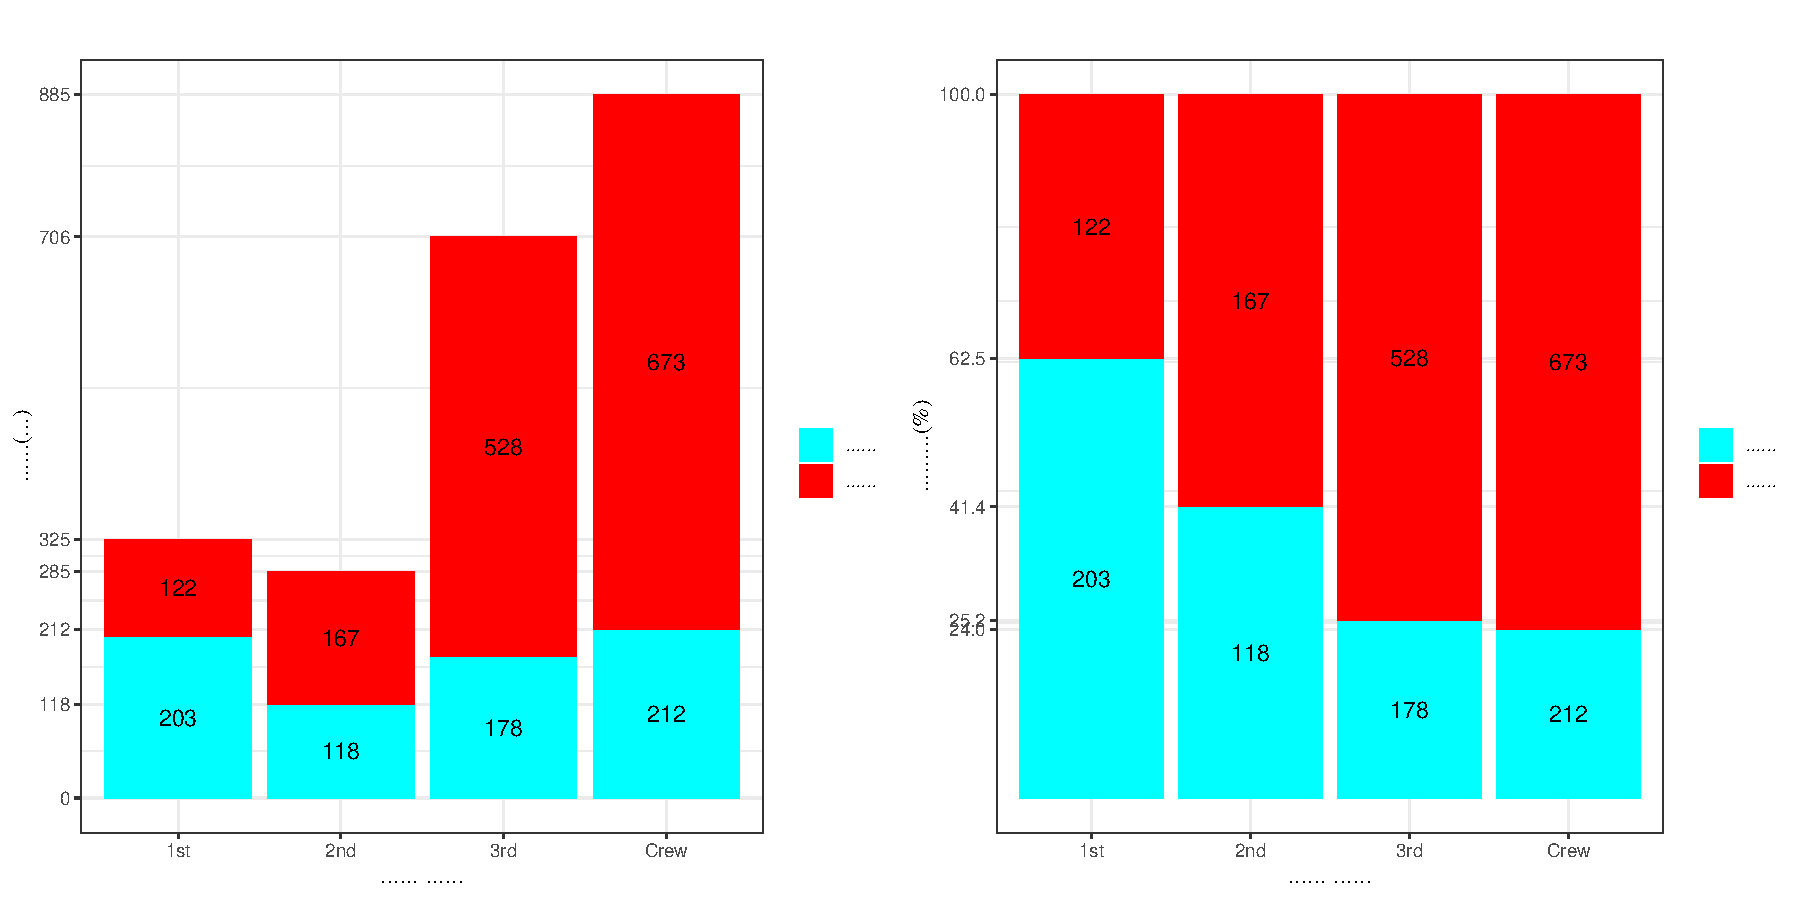
\includegraphics[width=0.75\linewidth]{Inequality_files/figure-latex/unnamed-chunk-4-1} \end{center}

\end{document}
